\scnsegmentheader{Описание реализации подсистемы взаимодействия с внешней средой с использованием сетевых языков}
\begin{scnsubstruct}

\scnheader{Реализация подсистемы взаимодействия с внешней средой с использованием сетевых языков}
\begin{scnrelfromlist}{компонент программной системы}
    \scnitem{Реализация подсистемы взаимодействия с внешней средой с использованием сетевых языков на основе языка JSON}
\end{scnrelfromlist}

\scntext{пояснение}{Взаимодействие программной модели sc-памяти с внешними ресурсами может осуществляться посредством специализированного программного интерфейса (API), однако этот вариант неудобен в большинстве случае, поскольку:
    \begin{scnitemize}
        \item поддерживается только для очень ограниченного набора языков программирования (С, С++);
        \item требует того, чтобы клиентское приложение, обращающееся к программной модели sc-памяти, фактически составляло с ней единое целое, таким образом исключается возможность построения распределенного коллектива ostis-систем;
        \item как следствие предыдущего пункта, исключается возможность параллельной работы с sc-памятью нескольких клиентских приложений.
    \end{scnitemize}
Для того, чтобы обеспечить возможность удаленного доступа к sc-памяти не учитывая при этом языки программирования, с помощью которых реализовано конкретное клиентское приложение, было принято решение о реализации возможности доступа к sc-памяти с использованием универсального языка, не зависящего от средств реализации того или иного компонента или системы. В качестве такого языка был разработан строковый язык на базе языка JSON.}

\scnstructheader{Описание подсистемы взаимодействия c sc-памятью на основе языка JSON}
\scnstartsubstruct

\scnheader{Реализация подсистемы взаимодействия c sc-памятью на основе языка JSON}
\scnexplanation{Реализация подсистемы взаимодействия c sc-памятью на основе языка JSON позволяет ostis-системам взаимодействовать с системами из внешней среды на основе общепринятого транспортного формата передачи данных JSON и предоставляет API для доступа к sc-памяти платформы интерпретации sc-моделей.}
\scnrelfromlist{используемый язык программирования}{C;C++;Python;TypeScript;CSharp;Java}
\scnrelfromlist{используемый язык}{SC-JSON-код}
\scnrelfrom{архитектура}{Клиент-серверная архитектура}
\scnrelto{реализация}{Подсистема взаимодействия с sc-памятью на основе языка JSON}
\scnaddlevel{1}
	\scnidtf{Подсистема взаимодействия с sc-памятью на основе формата JSON}
	\scnidtf{Подсистема взаимодействия с sc-памятью на основе транспортного формата передачи данных JSON}
	\scnexplanation{Взаимодействие c sc-памятью обеспечивается с помощью передачи информации на \textit{\textbf{SC-JSON-коде}} и ведётся, с одной стороны, между сервером, являющегося частью ostis-системы, написанным на том же языке реализации этой ostis-системы и имеющим доступ к её sc-памяти, и с другой стороны множеством клиентом, которым известно о наличии сервера в пределах сети их использования.}
	\scnnote{Осмысленные фрагменты текстов \textit{\textbf{SC-JSON-кода}} представляют семантически корректную структуру сущностей и связей между ними.}
	\scnnote{С помощью подсистемы взаимодействия с sc-памятью на основе языка JSON можно взаимодействовать с ostis-системой на таком же множестве возможных операций, как и в случае, если бы взаимодействие происходило (непосредственно) напрямую, на том же языке реализации платформы интерпретации sc-моделей компьютерных систем. При этом результат работы отличается только скоростью обработки информации.}
	\scnsubdividing{
		Серверная система на основе Websocket, обеспечивающая доступ к sc-памяти платформы интерпретации sc-моделей при помощи команд SC-JSON-кода\\;
		Множество клиентских систем, подключаемых и взаимодействующих с \textit{Серверной системой на основе Websocket, обеспечивающей доступ к sc-памяти платформы интерпретации sc-моделей при помощи команд SC-JSON-кода}\\
		\scnaddlevel{1}
			\scnsubdividing{
				Клиентская система, подключаемая и взаимодействующая с \textit{SC-сервером}, реализованная на языке программирования Python\\;
				Клиентская система, подключаемая и взаимодействующая с \textit{SC-сервером}, реализованная на языке программирования TypeScript\\;
				Клиентская система, подключаемая и взаимодействующая с \textit{SC-сервером}, реализованная на языке программирования CSharp\\;
				Клиентская система, подключаемая и взаимодействующая с \textit{SC-сервером}, реализованная на языке программирования Java
		}
		\scnaddlevel{-1}
}
\scnaddlevel{-1}

\scnheader{SC-JSON-код}
\scnidtf{Semantic JSON-code}
\scnidtf{Semantic JavaScript Object Notation code}
\scnidtf{Язык внешнего смыслового представления знаний для взаимодействия с ostis-системами на основе языка JSON}
\scnidtf{Метаязык, являющийся подмножеством языка JSON и обеспечивающий внешнее представление и структуризацию \textit{sc-текстов}, используемых ostis-системой в процессе своего функционирования и взаимодействия со внешней средой.}
\scntext{основной внешний идентификатор sc-элемента}{\textbf{SC-JSON-код}}
\scnaddlevel{1}
	\scniselement{имя собственное}
\scnaddlevel{-1}
\scntext{часто используемый неосновной внешний идентификатор sc-элемента}{sc-json-текст}
\scnaddlevel{1}
	\scniselement{имя нарицательное}
\scnaddlevel{-1}
\scniselement{абстрактный язык}
\scniselement{линейный язык}
\scnsuperset{JSON}
\filemodetrue
\scnrelfromvector{принципы, лежащие в основе}{
	Тексты, описываемые на языке внешнего представления знаний \textit{\textbf{SC-JSON-код}} представляют собой линейную структуру, представляемую в виде линейного строкового текста и состоящую из набора корректных осмысленных команд, записанных в виде \textit{sc-json-пар} вида \{отношение: объект\}, где отношением выступает знак квазибинарного отношения, состоящего из пар вида \{субъект: объект\}, где объектом выступает знак, обозначаемый предложением, включающее такие пары, а субъектом - sc-json-объекты: sc-json-литерал, sc-json-списки sc-json-объектов, sc-json-предложения, состоящие из sc-json-списков sc-json-объектов; 
	Тексты \textit{\textbf{SC-JSON-кода}} представляют собой sc-json-команды. Каждая команда представляет собой json-объект, в котором указываются уникальный идентификатор команды, тип этой команды и ее аргументы. C каждой командой ассоциируется ответ на эту команду. Ответ на команду представляет собой команду, в котором указываются идентификатор команды, ее статус (выполнена успешно/безуспешно) и результаты. Структура аргументов и результатов команды определяется типом команды. Для каждого ответа существует запрос.}
\filemodefalse 
\scnrelfromlist{достоинство}{
	\scnfileitem{Язык JSON является общепринятым открытым форматом, для работы с которым существует большое количество библиотек для популярных языков программирования. Это, в свою очередь, упрощает реализацию клиента и сервера для протокола, построенного на базе \textit{\textbf{SC-JSON-код}}.};
	\scnfileitem{Реализация подсистемы взаимодействия со внешней средой на базе \textit{\textbf{SC-JSON-код}} не накладывает принципиальных ограничений на объем (длину) каждой команды, в отличие от других бинарных протоколов. Таким образом, появляется возможность использования неатомарных команд, позволяющих, например, за один акт пересылки такой команды по сети создать сразу несколько sc-элементов. Важными примерами таких команд являются \textit{команда создания sc-конструкции, изоморфной заданному sc-шаблону}, и \textit{команда поиска sc-конструкций, изоморфных заданному sc-шаблону}.}}
\scnnote{Можно сказать, что язык на базе JSON является следующим шагом на пути к созданию мощного и универсального языка запросов, аналогичного языку SQL для реляционных баз данных и предназначенному для работы с sc-памятью. Следующий шагом станет реализация такого протокола на основе одного из стандартов внешнего отображения sc-конструкций, например, \textit{SCs-кода}, что, в свою очередь, позволит передавать в качестве команд целые программы обработки sc-конструкций, например на языке SCP.}

\scnstructheader{Синтаксис SC-JSON-кода}
\scnstartsubstruct
\scnheader{Синтаксис SC-JSON-кода}
\scnnote{\textit{Синтаксис SC-JSON-кода} задается: (1) \textit{Алфавитом SC-JSON-кода}, (2) Грамматикой SC-JSON-кода}
\scnrelto{синтаксис}{SC-JSON-код}

\scnstructheader{Синтаксическая классификация элементов SC-JSON-кода}
\scnstartsubstruct

\scnstructheader{SC-JSON-код}
\scnsubset{sc-json-предложение}
\scnaddlevel{1}
	\scnsubset{sc-json-список sc-json-пар}
	\scnaddlevel{1}
		\scnsuperset{sc-json-cписок}
		\scnsubset{sc-json-пара}
		\scnaddlevel{1}
			\scnsubset{sc-json-строка}
			\scnsubset{sc-json-объект}
			\scnaddlevel{1}
				\scnsubdividing
				{
					sc-json-cписок\\;
					sc-json-пара\\;
					sc-json-литерал\\
					\scnaddlevel{1}
						\scnsubdividing
						{
							sc-json-строка\\;
							sc-json-число
						}
					\scnaddlevel{-1}
				}
			\scnaddlevel{-1}
		\scnaddlevel{-1}
		\scnsubdividing
		{
			команда на SC-JSON-коде\\;
			ответ на команду на SC-JSON-коде
		}
	\scnaddlevel{-1}
\scnaddlevel{-1}

\scnendstruct \scninlinesourcecommentpar{Завершили представление \textit{Синтаксической классификации элементов SC-JSON-кода}}

\scnheader{Алфавит SC-JSON-кода\scnsupergroupsign}
\scnidtf{Множество всех возможных символов в SC-JSON-коде}
\scnexplanation{Поскольку SC-JSON-код является линейным строковым языком представления знаний, то его алфавит включает объединение алфавитов всех языков, тексты на которых могут представлять внешние идентификаторы и/или содержание sc-ссылок, множество всех цифр и множество всех других специальных символов.}
\scnrelto{алфавит}{SC-JSON-код}
\scnnote{Последовательности знаков алфавита могут образовывать sc-json ключевые слова, sc-json-пары, sc-json-предложения из sc-json-пар и sc-json-тексты из sc-json-предложений.}

\scnheader{SC-JSON-код}
\scnrelfromlist{синтаксические правила}{
	\scnfileitem{Каждое правило \textit{Грамматики SC-JSON-кода} описывает корректный с точки зрения \textit{Синтаксиса SC-JSON-кода} порядок sc-json-объектов в sc-json-предложении. Совокупность правил \textit{Грамматики SC-JSON-кода} описывает корректный с точки зрения \textit{Синтаксиса SC-JSON-кода} порядок sc-json-предложений в sc-json-тексте.};
	\scnfileitem{Каждое sc-json-предложение является sc-json-списком, состоящим из sc-json-пар и представляет собой команду или ответ на эту команду.};
	\scnfileitem{Каждое \textit{команда (ответ на команду) на SC-JSON-коде} состоит из заголовка, включающего sc-json-пары описания самой команды (ответа на команду), и сообщения, различного для каждого класса команд (ответов на команды). Сообщение {команды (ответа на команду) на SC-JSON-коде} обычно представляет собой список sc-json-объектов и может не ограничиваться по мощности.};
	\scnfileitem{Каждая sc-json-пара состоит из двух элементов: ключевого слова и некоторого другого sc-json-объекта, ассоциируемого с этим ключевым словом. Набор ключевых слов в sc-json-парах определяется конкретным классом {команд (ответов на команды) на SC-JSON-коде}. Sc-json-пара начинается знаком открывающейся фигурной скобки "\{" и заканчивается знаком закрывающейся фигурной скобки "\}". Ключевое слово и sc-json-объект, ассоциируемый с ним, разделяются при помощи знака двоеточия ":".};
	\scnfileitem{Sc-json-строки, записанные в sc-json-текстах, начинаются и заканчиваются знаком двух ковычек "\"{}".};
	\scnfileitem{Sc-json-списки, состоящие не из sc-json-пар, начинаются знаком открывающейся квадратной скобки "[" и заканчиваются знаком закрывающейся квадратной скобки "]". Sc-json-объектах в sc-json-списках разделяются запятыми ",".}
}

\scnheader{Грамматика SC-JSON-кода}
\scnidtf{Множество всех возможных правил, используемых при построении команд и ответов на них на SC-JSON-коде}
\scnexplanation{Каждой команде \textit{SC-JSON-кода} однозначно соответствует правило грамматики \textit{SC-JSON-кода}.}
\scnrelto{грамматика}{SC-JSON-код}
\scnexplanation{Правила \textit{Грамматики SC-JSON-кода} позволяют правильно составить команду на SC-JSON-коде, а также определить корректность запрашиваемой команды. Каждое правило грамматики \textit{SC-JSON-кода} представляется в виде правила на \textit{Языке описания грамматик ANTLR} и его интерпретации на естественном языке.}

\scnhaselementrole{ключевой sc-элемент}{Правило написания \textit{команд на SC-JSON-коде}}
\scnaddlevel{1}
	\scnrelfrom{обобщённая структура}{\scnfileimage{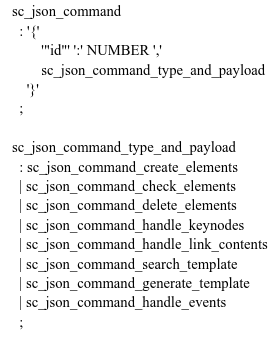
\includegraphics[scale=0.95]{images/command}}}
	\scnaddlevel{1}
		\scnsuperset{Язык описания грамматики языков ANTLR}
		\scnrelfromlist{интерпретация}{
		\scnfileitem{Класс \textit{команд на SC-JSON-коде} включает \textit{команду создания sc-элементов}, \textit{команду получения соответствующих типов sc-элементов}, \textit{команду удаления sc-элементов}, \textit{команду обработки ключевых sc-элементов}, \textit{команду обработки содержимого sc-ссылок}, \textit{команду поиска sc-конструкций, изоморфных заданному sc-шаблону}, \textit{команду генерации sc-конструкции, изоморфной заданному sc-шаблону}, и \textit{команду обработки sc-событий}. В \textit{команду на SC-JSON-коде} включаются идентификатор этой команды, тип и сообщение.}
	}
	\scnaddlevel{-1}
	\scnrelfrom{изоморфизм}{команда на SC-JSON-коде}
	\scnaddlevel{1}
		\scnidtf{sc-json-code command}
		\scnsuperset{SC-JSON-код}
		\scnnote{Множество \textit{команд на SC-JSON-коде} легко расширяемо засчёт гибкости и функциональности языка JSON.}
	\scnaddlevel{-1}
\scnaddlevel{-1}

\scnhaselement{Правило написания \textit{ответов на команды на SC-JSON-коде}}
\scnaddlevel{1}
	\scnrelfrom{обобщённая структура}{\scnfileimage{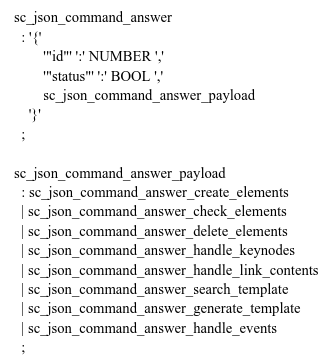
\includegraphics[scale=0.95]{images/command_answer}}}
	\scnaddlevel{1}
		\scnsuperset{Язык описания грамматики языков ANTLR}
		\scnrelfromlist{интерпретация}{
			\scnfileitem{Класс \textit{ответов на команды на SC-JSON-коде} включает \textit{ответ на команду создания sc-элементов}, \textit{ответ на команду получения соответствующих типов sc-элементов}, \textit{ответ на команду удаления sc-элементов}, \textit{ответ на команду обработки ключевых sc-элементов}, \textit{ответ на команду обработки содержимого sc-ссылок}, \textit{ответ на команду поиска sc-конструкций, изоморфных заданному sc-шаблону}, \textit{ответ на команду генерации sc-конструкции, изоморфной заданному sc-шаблону}, и \textit{ответ на команду обработки sc-событий}. В \textit{ответ на команду на SC-JSON-коде} включаются идентификатор соответствующей команды, статус обработки ответа и ответное сообщение.}
		}
	\scnaddlevel{-1}
	\scnrelfrom{изоморфизм}{команда на SC-JSON-коде}
	\scnaddlevel{1}
		\scnidtf{sc-json-code command}
		\scnsuperset{SC-JSON-код}
		\scnnote{Каждой команде на SC-JSON-коде однозначно соответствует ответ на эту команду на SC-JSON-коде.}
	\scnaddlevel{-1}
\scnaddlevel{-1}

\scnhaselement{Правило написания \textit{команды создания sc-элементов}}
\scnaddlevel{1}
	\scnrelfrom{обобщённая структура}{\scnfileimage{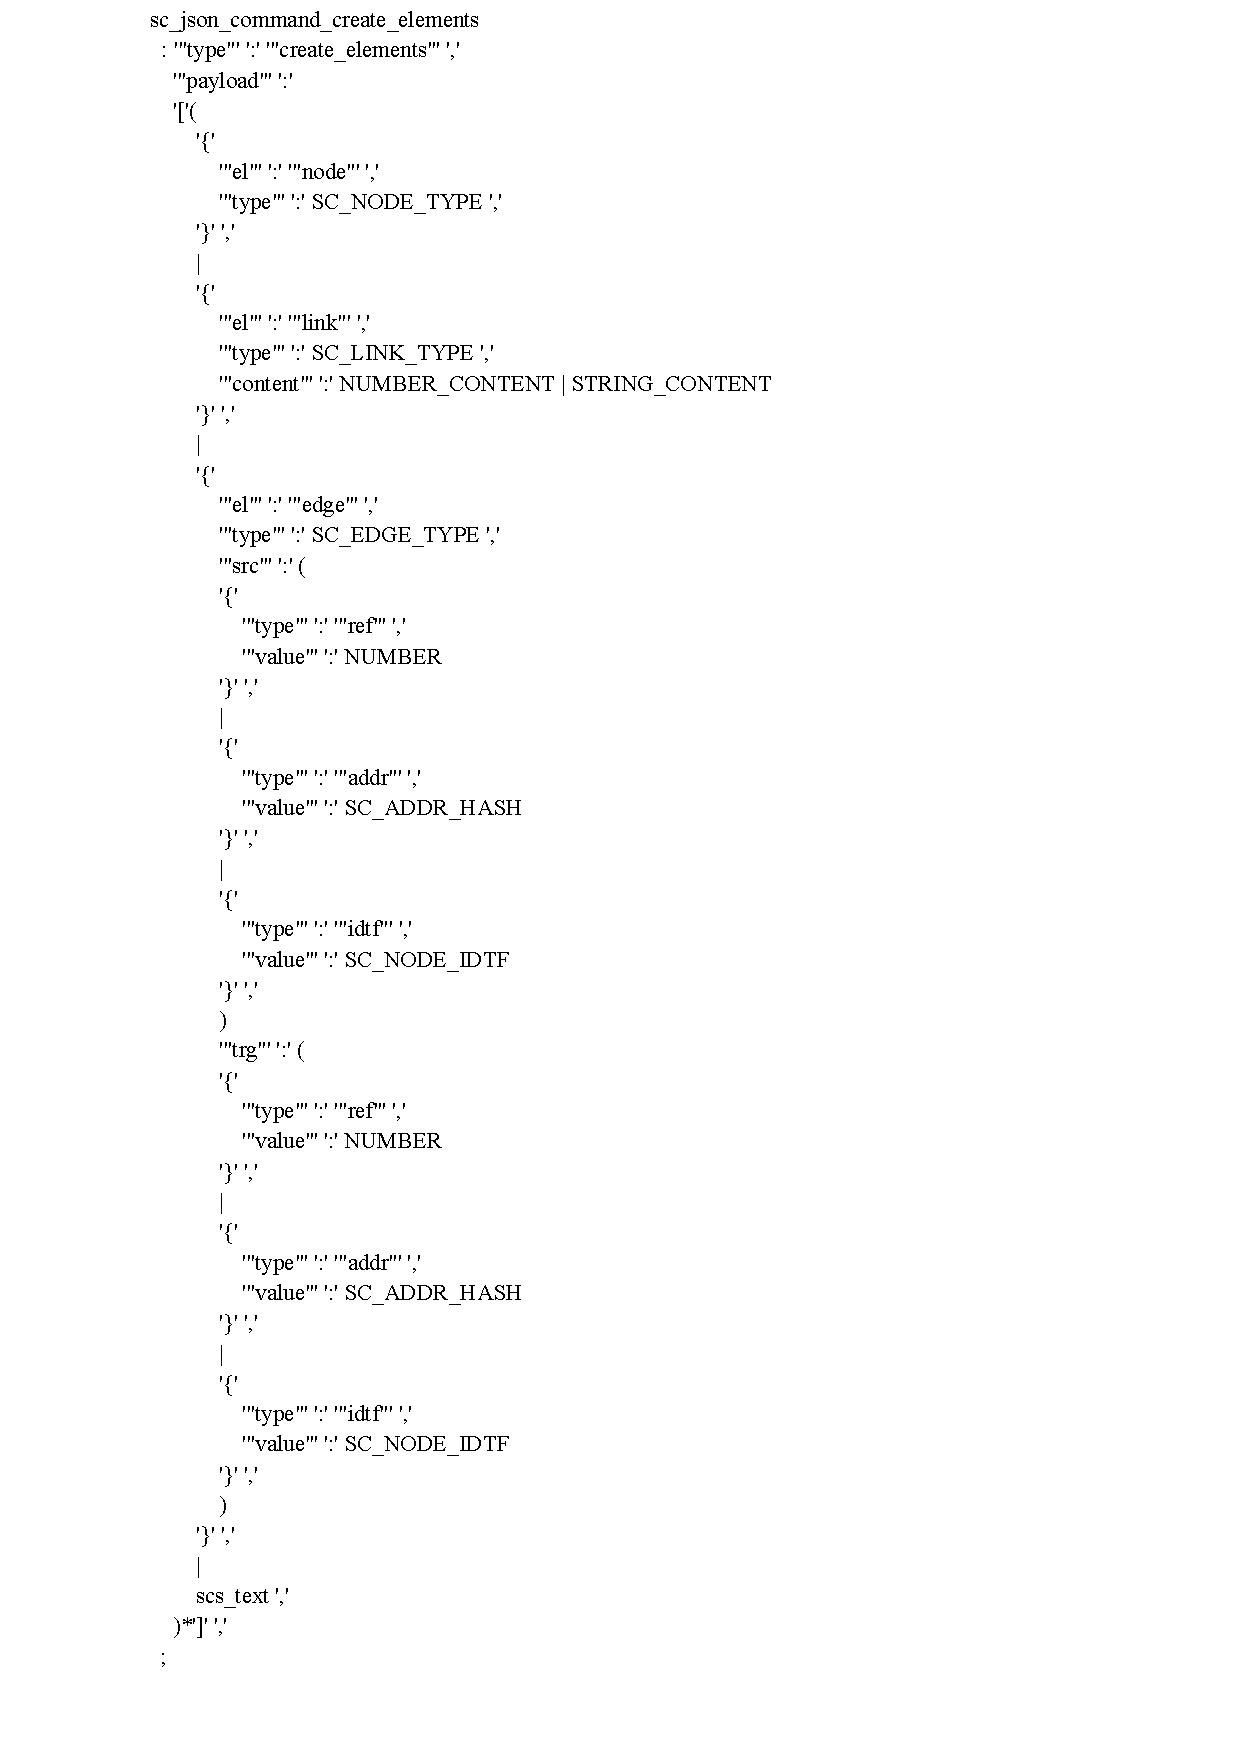
\includegraphics[scale=0.95]{images/create_elements_command}}}
	\scnaddlevel{1}
		\scnsuperset{Язык описания грамматики языков ANTLR}
		\scnrelfromlist{интерпретация}{
			\scnfileitem{В сообщении \textit{команды создания sc-элементов} представляется список описаний создаваемых sc-элементов. Такими sc-элементами могут быть sc-узел, sc-дуга, sc-ребро или sc-ссылка. Тип sc-элемента указывается в паре с ключевым словом "el": для sc-узла sc-json-тип элемент представляется как "node"{}, для sc-дуги и sc-ребра - "edge"{}, для sc-ссылки - "link". Метки типов sc-элементов уточняются в соответствующих им описаниях в сообщении команды в паре с ключевым словом "type". Если создаваемым sc-элементом является sc-ссылка, то дополнительно указывается содержимое этой sc-ссылки в паре с ключевым словом "content", если создаваемым sc-элементом является sc-дуга или sc-ребро, то указываются описания sc-элементов, из которых они выходят, и sc-элементов, в которые они входят. Описание таких sc-элементов состоят из двух пар: первая пара указывает на способ ассоциации с sc-элементом и представляется как "addr"{} или "idtf"{} или "ref"{} в паре с ключевым словом "type"{}, вторая пара - то, по чему происходит ассоциация с этим sc-элементом: его хешу, системному идентификатору или номеру в массиве создаваемых sc-элементов - в паре с ключевым словом "value".}
		}
	\scnaddlevel{-1}
	\scnrelfrom{изоморфизм}{команда создания sc-элементов}
	\scnaddlevel{1}
		\scnidtf{create elements command}
		\scnsuperset{команда на SC-JSON-коде}
		\scnsuperset{SC-JSON-код}
		\scnrelfrom{пример}{Пример команды создания sc-элементов \\ \scneqfile{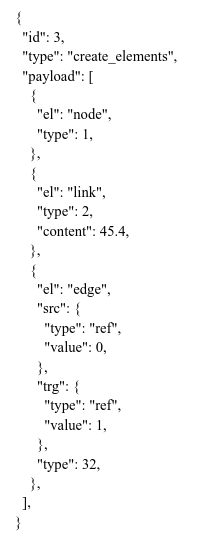
\includegraphics[scale=0.95]{images/create_elements_command_example}}}
		\scnaddlevel{1}
			\scniselement{команда создания sc-элементов}
			\scnrelfrom{ответ}{Пример ответа на команду создания sc-элементов}
			\scnrelfromlist{интерпретация}{
				\scnfileitem{Обработать команду создания sc-элементов: sc-узла с типом 1 (неуточняемого типа), sc-ссылки с типом 2 (неуточняемого типа) и содержимым в виде числа с плавающей точкой 45.4 и sc-дуги типа 32 (константного типа) между sc-элементом, находящимся на нулевой позиции в массиве создаваемых sc-элементов, и sc-элементом, находящимся на первой позиции в том же самом массиве.}
			}
		\scnaddlevel{-1}
		\scnrelfrom{ответная структура}{ответ на команду создания sc-элементов}
		\scnnote{Стоит отметить, что на уровне интерфейса sc-памяти команда интерпретируется быстро за счёт того, что не используются шаблоны создания изоморфных им конструкций. Также содержимое сообщения \textit{команды создания sc-элементов} может быть пустым.}
	\scnaddlevel{-1}
\scnaddlevel{-1}

\scnhaselement{Правило написания \textit{ответа на команду создания sc-элементов}}
\scnaddlevel{1}
	\scnrelfrom{обобщённая структура}{\scnfileimage{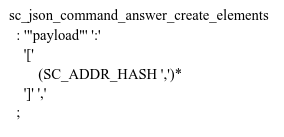
\includegraphics[scale=0.95]{images/create_elements_command_answer}}}
	\scnaddlevel{1}
		\scnsuperset{Язык описания грамматики языков ANTLR}
		\scnrelfromlist{интерпретация}{
			\scnfileitem{Сообщением \textit{ответа на команду создания sc-элементов} является список хешей созданных sc-элементов, соответствующих описаниям \textit{команды создания sc-элементов} со статусом 1, в случае успешной обработки команды.}
		}
	\scnaddlevel{-1}
	\scnrelfrom{изоморфизм}{ответ на команду создания sc-элементов}
	\scnaddlevel{1}
		\scnidtf{create elements command answer}
		\scnsuperset{ответ на команду на SC-JSON-коде}
		\scnsuperset{SC-JSON-код}
		\scnrelfrom{пример}{Пример ответа на команду создания sc-элементов \\ \scneqfile{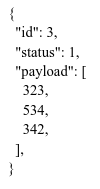
\includegraphics[scale=0.95]{images/create_elements_command_answer_example}}}
		\scnaddlevel{1}
			\scniselement{ответ на команду создания sc-элементов}
			\scnrelfromlist{интерпретация}{
				\scnfileitem{Созданы sc-элементы с хешами 323, 534 и 342 соответственно. Команда обработана успешно.}
			}
		\scnaddlevel{-1}
	\scnaddlevel{-1}
\scnaddlevel{-1}

\scnhaselement{Правило написания \textit{команды получения соответствующих типов sc-элементов}}
\scnaddlevel{1}
	\scnrelfrom{обобщённая структура}{\scnfileimage{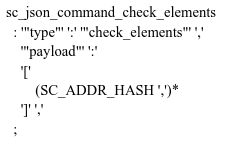
\includegraphics[scale=0.95]{images/check_elements_command}}}
	\scnaddlevel{1}
		\scnsuperset{Язык описания грамматики языков ANTLR}
		\scnrelfromlist{интерпретация}{
			\scnfileitem{Сообщением \textit{команды получения соответствующих типов sc-элементов} является списком хешей sc-элементов, у которых необходимо получить синтаксические типы.}
		}
	\scnaddlevel{-1}
	\scnrelfrom{изоморфизм}{команда получения соответствующих типов sc-элементов}
	\scnaddlevel{1}
		\scnidtf{check elements command}
		\scnsuperset{команда на SC-JSON-коде}
		\scnsuperset{SC-JSON-код}
		\scnrelfrom{пример}{Пример команды получения соответствующих типов sc-элементов \\ \scneqfile{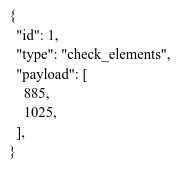
\includegraphics[scale=0.95]{images/check_elements_command_example}}}
		\scnaddlevel{1}
			\scniselement{команда получения соответствующих типов sc-элементов}
			\scnrelfrom{ответ}{Пример ответа на команду получения соответствующих типов sc-элементов}
			\scnrelfromlist{интерпретация}{
				\scnfileitem{Получить синтаксические типы sc-элементов с хешами 885 и 1025.}
			}
		\scnaddlevel{-1}
		\scnrelfrom{ответная структура}{ответ на команду получения соответствующих типов sc-элементов}
		\scnnote{
		Содержимое сообщения \textit{команды получения соответствующих типов sc-элементов} может быть пустым.
		}
	\scnaddlevel{-1}
\scnaddlevel{-1}

\scnhaselement{Правило написания \textit{ответа на команду получения соответствующих типов sc-элементов}}
\scnaddlevel{1}
	\scnrelfrom{обобщённая структура}{\scnfileimage{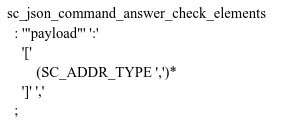
\includegraphics[scale=0.95]{images/check_elements_command_answer}}}
	\scnaddlevel{1}
		\scnsuperset{Язык описания грамматики языков ANTLR}
		\scnrelfromlist{интерпретация}{
		\scnfileitem{Сообщением \textit{ответа на команду получения соответствующих типов sc-элементов} является список типов проверенных sc-элементов, соответствующих описаниям \textit{команды получения соответствующих типов sc-элементов} со статусом 1, в случае успешной обработки команды.}
	}
	\scnaddlevel{-1}
	\scnrelfrom{изоморфизм}{ответ на команду получения соответствующих типов sc-элементов}
	\scnaddlevel{1}
		\scnidtf{check elements command answer}
		\scnsuperset{ответ на команду на SC-JSON-коде}
		\scnsuperset{SC-JSON-код}
		\scnrelfrom{пример}{Пример ответа на команду получения соответствующих типов sc-элементов \\ \scneqfile{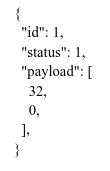
\includegraphics[scale=0.95]{images/check_elements_command_answer_example}}}
		\scnaddlevel{1}
			\scniselement{ответ на команду получения соответствующих типов sc-элементов}
			\scnrelfromlist{интерпретация}{
				\scnfileitem{Типы sc-элементов 32 и 0 соответственно. Команда обработана успешно.}
			}
		\scnaddlevel{-1}
		\scnnote{Если sc-элемент с указанным хешем не существует, то его тип будет равен 0.}
	\scnaddlevel{-1}
\scnaddlevel{-1}

\scnhaselement{Правило написания \textit{команды удаления sc-элементов}}
\scnaddlevel{1}
	\scnrelfrom{обобщённая структура}{\scnfileimage{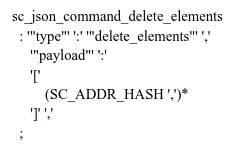
\includegraphics[scale=0.95]{images/delete_elements_command}}}
	\scnaddlevel{1}
		\scnsuperset{Язык описания грамматики языков ANTLR}
		\scnrelfromlist{интерпретация}{
			\scnfileitem{Сообщением \textit{команды удаления sc-элементов} является список хешей sc-элементов, которые необходимо удалить из sc-памяти.}
		}
	\scnaddlevel{-1}
	\scnrelfrom{изоморфизм}{команда удаления sc-элементов}
	\scnaddlevel{1}
		\scnidtf{delete elements command}
		\scnsuperset{команда на SC-JSON-коде}
		\scnsuperset{SC-JSON-код}
		\scnrelfrom{пример}{Пример команды удаления sc-элементов \\ \scneqfile{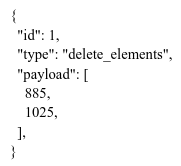
\includegraphics[scale=0.95]{images/delete_elements_command_example}}}
		\scnaddlevel{1}
			\scniselement{команда удаления sc-элементов}
			\scnrelfrom{ответ}{Пример ответа на команду удаления sc-элементов}
			\scnrelfromlist{интерпретация}{
				\scnfileitem{Удалить sc-элементы с хешами 885 и 1025.}
			}
		\scnaddlevel{-1}
		\scnrelfrom{ответная структура}{ответ на команду удаления sc-элементов}
		\scnnote{Содержимое сообщения \textit{команды удаления sc-элементов} может быть пустым.}
	\scnaddlevel{-1}
\scnaddlevel{-1}

\scnhaselement{Правило написания \textit{ответа на команду удаления sc-элементов}}
\scnaddlevel{1}
	\scnrelfrom{обобщённая структура}{\scnfileimage{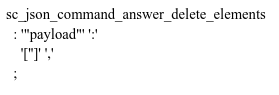
\includegraphics[scale=0.95]{images/delete_elements_command_answer}}}
	\scnaddlevel{1}
		\scnsuperset{Язык описания грамматики языков ANTLR}
		\scnrelfromlist{интерпретация}{
			\scnfileitem{Сообщение \textit{ответа на команду удаления sc-элементов} является пустым со статусом 1, в случае успешной обработки команды.}
		}
	\scnaddlevel{-1}
	\scnrelfrom{изоморфизм}{ответ на команду удаления sc-элементов}
	\scnaddlevel{1}
		\scnidtf{delete elements command answer}
		\scnsuperset{ответ на команду на SC-JSON-коде}
		\scnsuperset{SC-JSON-код}
		\scnrelfrom{пример}{Пример ответа на команду удаления sc-элементов \\ \scneqfile{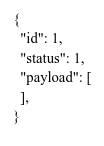
\includegraphics[scale=0.95]{images/delete_elements_command_answer_example}}}
		\scnaddlevel{1}
			\scniselement{ответ на команду удаления sc-элементов}
			\scnrelfromlist{интерпретация}{
				\scnfileitem{Sc-элементы были удалены из sc-памяти успешно.}
			}
		\scnaddlevel{-1}
		\scnnote{Если sc-элемент с указанным хешем не существует, ответ на команду будет безуспешным.}
	\scnaddlevel{-1}
\scnaddlevel{-1}

\scnhaselement{Правило написания \textit{команды обработки ключевых sc-элементов}}
\scnaddlevel{1}
	\scnrelfrom{обобщённая структура}{\scnfileimage{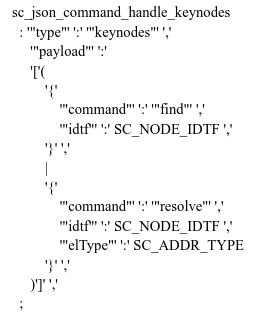
\includegraphics[scale=0.95]{images/handle_keynodes_command}}}
	\scnaddlevel{1}
	\scnsuperset{Язык описания грамматики языков ANTLR}
	\scnrelfromlist{интерпретация}{
		\scnfileitem{Сообщение \textit{команды обработки ключевых sc-элементов} может включать описание ключевых sc-элементов, которые необходимо найти и/или разрешить по их идентификаторам. Такое деление осуществляется с помощью подкоманд, содержащихся в сообщении команды. Идентификаторами подкоманд могут быть "find"{} и "resolve"{} соответственно, стоящие в паре с ключевым словом "command". Описание искомого sc-элемента команды "find"{} включает системный идентификатор sc-элемента, по которому необходимо найти этот sc-элемент, стоящий в паре с ключевым словом "idtf". Описание разрешаемого sc-элемента команды "resolve"{} включает системный идентификатор sc-элемента, по которому необходимо найти этот sc-элемент, либо в случае безуспешного поиска создать sc-элемент некоторого типа, указанного в его описании в паре с ключевым словом "elType"{}, и установить для него системный идентификатор, по которому была произведена попытка найти другой sc-элемент.}
	}
	\scnaddlevel{-1}
	\scnrelfrom{изоморфизм}{команда обработки ключевых sc-элементов}
	\scnaddlevel{1}
		\scnidtf{handle keynodes command}
		\scnsuperset{команда на SC-JSON-коде}
		\scnsuperset{SC-JSON-код}
		\scnrelfrom{пример}{Пример команды обработки ключевых sc-элементов \\ \scneqfile{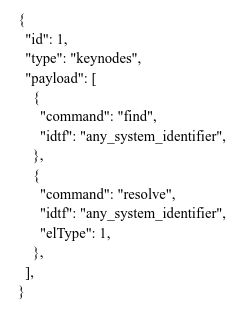
\includegraphics[scale=0.95]{images/handle_keynodes_command_example}}}
		\scnaddlevel{1}
		\scniselement{команда обработки ключевых sc-элементов}
		\scnrelfrom{ответ}{Пример ответа на команду обработки ключевых sc-элементов}
		\scnrelfromlist{интерпретация}{
			\scnfileitem{(1) Найти sc-элемент по системному идентификатору "any\_system\_identifier"{}; (2) Разрешить sc-элемент с типом 1 (неуточняемого типа) по системному идентификатору "any\_system\_identifier"{}.}
		}
		\scnaddlevel{-1}
		\scnrelfrom{ответная структура}{ответ на команду обработки ключевых sc-элементов}
		\scnnote{Данный класс команд позволяет быстро обращаться к sc-элементам по их системным идентификаторам, поскольку ключевые sc-элементы 	кэшируются на уровне интерфейса.}
	\scnaddlevel{-1}
\scnaddlevel{-1}

\scnhaselement{Правило написания \textit{ответа на команду обработки ключевых sc-элементов}}
\scnaddlevel{1}
	\scnrelfrom{обобщённая структура}{\scnfileimage{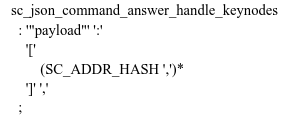
\includegraphics[scale=0.95]{images/handle_keynodes_command_answer}}}
	\scnaddlevel{1}
	\scnsuperset{Язык описания грамматики языков ANTLR}
	\scnrelfromlist{интерпретация}{
		\scnfileitem{Сообщением \textit{ответа на команду обработки ключевых sc-элементов} является список хешей sc-элементов, соответствующих описаниям \textit{команды обработки ключевых sc-элементов} со статусом 1, в случае успешной обработки команды.}
	}
	\scnaddlevel{-1}
	\scnrelfrom{изоморфизм}{ответ на команду обработки ключевых sc-элементов}
	\scnaddlevel{1}
		\scnidtf{handle keynodes command answer}
		\scnsuperset{ответ на команду на SC-JSON-коде}
		\scnsuperset{SC-JSON-код}
		\scnrelfrom{пример}{Пример ответа на команду обработки ключевых sc-элементов \\ \scneqfile{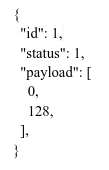
\includegraphics[scale=0.95]{images/handle_keynodes_command_answer_example}}}
		\scnaddlevel{1}
			\scniselement{ответ на команду обработки ключевых sc-элементов}
			\scnrelfromlist{интерпретация}{
				\scnfileitem{Ключевый sc-элемент с системным идентификатором "any\_system\_identifier"{} не был найден, поэтому был создан. Хеш нового ключевого sc-элемента - 128. Команда выполнена 	успешно.}
			}
		\scnaddlevel{-1}
	\scnaddlevel{-1}
\scnaddlevel{-1}

\scnhaselement{Правило написания \textit{команды обработки содержимого sc-ссылок}}
\scnaddlevel{1}
	\scnrelfrom{обобщённая структура}{\scnfileimage{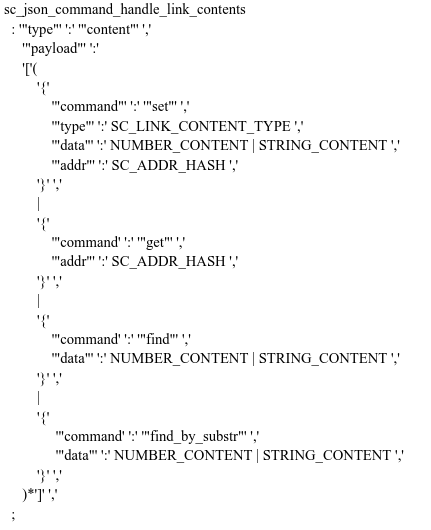
\includegraphics[scale=0.95]{images/handle_link_contents_command}}}
	\scnaddlevel{1}
		\scnsuperset{Язык описания грамматики языков ANTLR}
		\scnrelfromlist{интерпретация}{
			\scnfileitem{Сообщение \textit{команды обработки содержимого sc-ссылок} может включать описание ключевых sc-ссылок, которые необходимо найти по их содержимому, для которых необходимо установить содержимое разрешить и/или у которых необходимо получить содержимое. Как и в \textit{Правиле написания команды обработки ключевых sc-элементов} деление осуществляется с помощью подкоманд, содержащихся в сообщении команды. Идентификаторами подкоманд могут быть "find"{}, "set"{} и "get"{} соответственно, стоящие в паре с ключевым словом "command". В описаниях команд "set"{} и "get"{} указывается хеш sc-ссылки в паре с ключевым словом "addr". В описаниях команд "set"{} и "find"{} указывается содержимое sc-ссылки в паре с ключевым словом "data". Дополнительно в описании подкоманды "set"{} указывается тип устанавливаемого содержимого sc-ссылки.}
		}
	\scnaddlevel{-1}
	\scnrelfrom{изоморфизм}{команда обработки содержимого sc-ссылок}
	\scnaddlevel{1}
		\scnidtf{handle link contents command}
		\scnsuperset{команда на SC-JSON-коде}
		\scnsuperset{SC-JSON-код}
		\scnrelfrom{пример}{Пример команды обработки содержимого sc-ссылок \\ \scneqfile{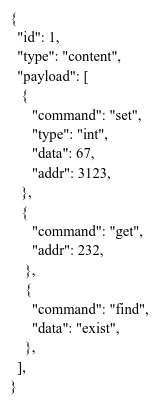
\includegraphics[scale=0.95]{images/handle_link_contents_command_example}}}
		\scnaddlevel{1}
			\scniselement{команда обработки содержимого sc-ссылок}
			\scnrelfrom{ответ}{Пример ответа на команду обработки содержимого sc-ссылок}
			\scnrelfromlist{интерпретация}{
				\scnfileitem{(1) Установить содержимое 67 типа "int"{} в sc-ссылку с хешем 3123; (2) Получить содержимое sc-ссылки с хешем 232; (3) Найти sc-ссылки с содержимым "exist"{}.}
			}
		\scnaddlevel{-1}
		\scnrelfrom{ответная структура}{ответ на команду обработки содержимого sc-ссылок}
		\scnnote{Стоит отметить, что в случае, если sc-ссылка уже имеет содержимое, то при установке нового содержимого старое содержимое будет удалено из памяти. Содержимое sc-ссылки может быть установлено как пустое.}
	\scnaddlevel{-1}
\scnaddlevel{-1}

\scnhaselement{Правило написания \textit{ответа на команду обработки содержимого sc-ссылок}}
\scnaddlevel{1}
	\scnrelfrom{обобщённая структура}{\scnfileimage{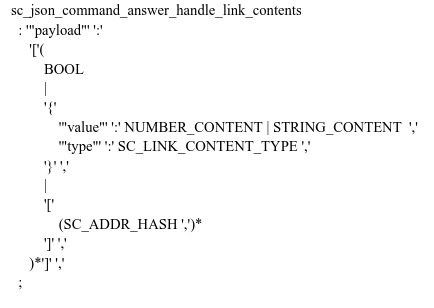
\includegraphics[scale=0.95]{images/handle_link_contents_command_answer}}}
	\scnaddlevel{1}
		\scnsuperset{Язык описания грамматики языков ANTLR}
		\scnrelfromlist{интерпретация}{
			\scnfileitem{Сообщением \textit{ответа на команду обработки содержимого sc-ссылок} является список, состоящий из булевого результата установки содержимого в sc-ссылку и/или найденных sc-ссылок по их содержимому и/или описания полученного содержимого sc-ссылок, соответствующих описаниям \textit{команды обработки содержимого sc-ссылок} со статусом 1, в случае успешной обработки команды.}
		}
	\scnaddlevel{-1}
	\scnrelfrom{изоморфизм}{ответ на команду обработки содержимого sc-ссылок}
	\scnaddlevel{1}
		\scnidtf{handle link contents command answer}
		\scnsuperset{ответ на команду на SC-JSON-коде}
		\scnsuperset{SC-JSON-код}
		\scnrelfrom{пример}{Пример ответа на команду обработки содержимого sc-ссылок \\ \scneqfile{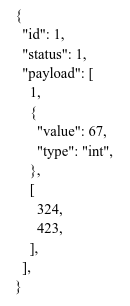
\includegraphics[scale=0.95]{images/handle_link_contents_command_answer_example}}}
		\scnaddlevel{1}
			\scniselement{ответ на команду обработки содержимого sc-ссылок}
			\scnrelfromlist{интерпретация}{
				\scnfileitem{(1) Содержимое 67 типа "int"{} было установлено успешно в sc-ссылку с хешем 3123; (2) Содержимое sc-ссылки с хешем 232 - число 67 целочисленного типа; (3) Sc-ссылки с содержимым "exist"{}: 324 и 423.}
			}
		\scnaddlevel{-1}
	\scnaddlevel{-1}
\scnaddlevel{-1}

\scnhaselement{Правило написания \textit{команды поиска sc-конструкций, изоморфных заданному sc-шаблону}}
\scnaddlevel{1}
	\scnrelfrom{обобщённая структура}{\scnfileimage{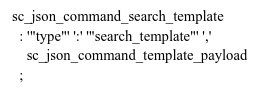
\includegraphics[scale=0.95]{images/search_template_command}}}
	\scnaddlevel{1}
		\scnsuperset{Язык описания грамматики языков ANTLR}
		\scnsubset{Правило написания сообщения \textit{команды поиска sc-конструкций, изоморфных заданному sc-шаблону}, и \textit{команды генерации sc-конструкции, изоморфной заданному sc-шаблону}}
		\scnrelfromlist{интерпретация}{
			\scnfileitem{\textit{Правило написания команды поиска sc-конструкций, изоморфных заданному sc-шаблону} включает \textit{Правило написания сообщения \textit{команды поиска sc-конструкций, изоморфных заданному sc-шаблону,} и \textit{команды генерации sc-конструкции, изоморфной заданному sc-шаблону}} и описывает команду поиска sc-конструкций по сформированному этой командой sc-шаблону (см. \textit{Правило написания сообщения \textit{команды поиска sc-конструкций, изоморфных заданному sc-шаблону,} и \textit{команды генерации sc-конструкции, изоморфной заданному sc-шаблону}}).}
		}
	\scnaddlevel{-1}
	\scnrelfrom{изоморфизм}{команда поиска sc-конструкций, изоморфных заданному sc-шаблону}
	\scnaddlevel{1}
		\scnidtf{search template command}
		\scnsuperset{команда на SC-JSON-коде}
		\scnsuperset{SC-JSON-код}
		\scnrelfrom{пример}{Пример команды поиска sc-конструкций, изоморфных заданному sc-шаблону \\ \scneqfile{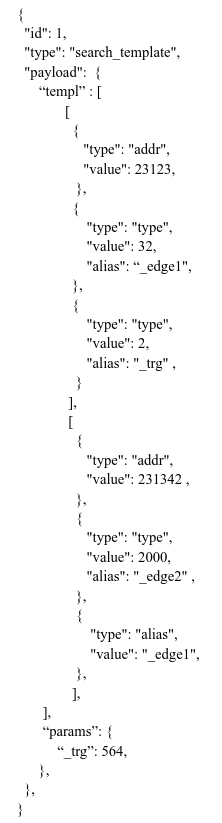
\includegraphics[scale=0.95]{images/search_template_command_example}}}
		\scnaddlevel{1}
			\scniselement{команда поиска sc-конструкций, изоморфных заданному sc-шаблону}
			\scnrelfrom{ответ}{Пример ответа на команду поиска sc-конструкций, изоморфных заданному sc-шаблону}
			\scnrelfromlist{интерпретация}{
				\scnfileitem{Найти все такие тройки, в которых первым элементом является sc-элемент c хешем 23123, третьим sc-элементом является sc-cсылка неуточняемого константного типа c псевдонимом “\_trg”{}, а вторым элементом - sc-дуга типа sc\_edge\_d\_common c псевдонимом “\_edge1”{}, исходящая от sc-элемента c хешем 23123 и входящая в sc-ссылку с псевдонимом “\_trg”{}, и найти все такие тройки, в которых первым элементом является sc-элемент c хешем 231342, третьим элементов является sc-дуга под псевдонимом “\_edge1”{}, а вторым элементом - sc-дуга типа sc\_edge\_access\_const\_pos\_perm, исходящая от sc-элемента c хешем 231342 и входящая в sc-дугу “\_edge1”. На место переменной с псевдонимом “\_trg”{} подставить sc-элемент с хешем 564.}
			}
		\scnaddlevel{-1}
		\scnrelfrom{ответная структура}{ответ на команду поиска sc-конструкций, изоморфных заданному sc-шаблону}
		\scnnote{Поиск sс-конструкций по сформированному sc-шаблону осуществляется специализированным модулем, являющимся частью sc-памяти.}
	\scnaddlevel{-1}
\scnaddlevel{-1}

\scnhaselement{Правило написания \textit{ответа на команду поиска sc-конструкций, изоморфных заданному sc-шаблону}}
\scnaddlevel{1}
	\scnrelfrom{обобщённая структура}{\scnfileimage{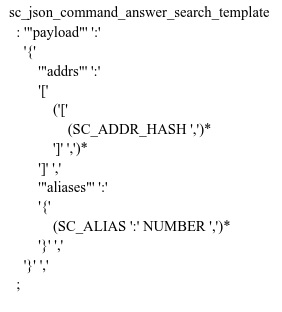
\includegraphics[scale=0.95]{images/search_template_command_answer}}}
	\scnaddlevel{1}
		\scnsuperset{Язык описания грамматики языков ANTLR}
		\scnrelfromlist{интерпретация}{
			\scnfileitem{Сообщение \textit{ответа на команду поиска sc-конструкций, изоморфных заданному sc-шаблону} состоит из списка найденных sc-конструкций и отображения псевдонимов sc-элементов на их позиции в тройках sc-шаблона. Ответ имеет статус 1, в случае успешной обработки команды.}
		}
	\scnaddlevel{-1}
	\scnrelfrom{изоморфизм}{ответ на команду поиска sc-конструкций, изоморфных заданному sc-шаблону}
	\scnaddlevel{1}
		\scnidtf{search template command answer}
		\scnsuperset{ответ на команду на SC-JSON-коде}
		\scnsuperset{SC-JSON-код}
		\scnrelfrom{пример}{Пример ответа на команду поиска sc-конструкций, изоморфных заданному sc-шаблону \\ \scneqfile{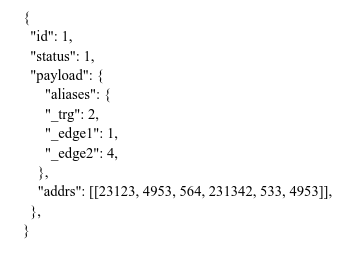
\includegraphics[scale=0.95]{images/search_template_command_answer_example}}}
		\scnaddlevel{1}
			\scniselement{ответ на команду поиска sc-конструкций, изоморфных заданному sc-шаблону}
			\scnrelfromlist{интерпретация}{
			\scnfileitem{Найдена одна sc-конструкция, состоящая из двух троек. Хеши sc-элементов в тройках: 23123, 4953, 564 и 231342, 533, 4953 соответственно их расположению в тройках. Команда выполнена успешно.}
		}
		\scnaddlevel{-1}
		\scnnote{Важно отметить, что sc-шаблон поиска sc-конструкций не может быть пустым.}
	\scnaddlevel{-1}
\scnaddlevel{-1}

\scnhaselement{Правило написания \textit{команды создания sc-конструкции, изоморфной заданному sc-шаблону}}
\scnaddlevel{1}
	\scnrelfrom{обобщённая структура}{\scnfileimage{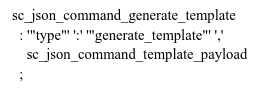
\includegraphics[scale=0.95]{images/generate_template_command}}}
	\scnaddlevel{1}
		\scnsuperset{Язык описания грамматики языков ANTLR}
		\scnsubset{Правило написания сообщения \textit{команды поиска sc-конструкций, изоморфных заданному sc-шаблону,} и \textit{команды генерации sc-конструкции, изоморфной заданному sc-шаблону}}
		\scnrelfromlist{интерпретация}{
			\scnfileitem{\textit{Правило написания команды создания sc-конструкции, изоморфной заданному sc-шаблону} включает \textit{Правило написания сообщения \textit{команды поиска sc-конструкций, изоморфных заданному sc-шаблону,} и \textit{команды генерации sc-конструкции, изоморфной заданному sc-шаблону}} и описывает команду создания sc-конструкции по сформированному этой командой sc-шаблону (см. \textit{Правило написания сообщения \textit{команды поиска sc-конструкций, изоморфных заданному sc-шаблону,} и \textit{команды генерации sc-конструкции, изоморфной заданному sc-шаблону}}).}
		}
	\scnaddlevel{-1}
	\scnrelfrom{изоморфизм}{команда создания sc-конструкции, изоморфной заданному sc-шаблону}
	\scnaddlevel{1}
		\scnidtf{generate template command}
		\scnsuperset{команда на SC-JSON-коде}
		\scnsuperset{SC-JSON-код}
		\scnrelfrom{пример}{Пример команды создания sc-конструкции, изоморфной заданному sc-шаблону \\ \scneqfile{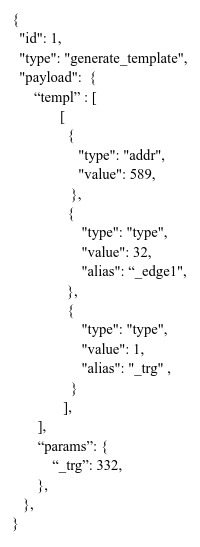
\includegraphics[scale=0.95]{images/generate_template_command_example}}}
		\scnaddlevel{1}
			\scniselement{команда создания sc-конструкции, изоморфной заданному sc-шаблону}
			\scnrelfrom{ответ}{Пример ответа на команду создания sc-конструкции, изоморфной заданному sc-шаблону}
			\scnrelfromlist{интерпретация}{
				\scnfileitem{Создать такую тройку, в которой первым элементом является sc-элемент c хешем 589, третьим sc-элементом является sc-узел неуточняемого типа c псевдонимом “\_trg”{}, а вторым элементом - sc-дуга типа sc\_edge\_d\_common c псевдонимом “\_edge1”{}, исходящая от sc-элемента c хешем 589 и входящая в sc-узел с псевдонимом “\_trg”{}. На место переменной с псевдонимом “\_trg”{} подставить sc-элемент с хешем 332.}
			}
		\scnaddlevel{-1}
		\scnrelfrom{ответная структура}{ответ на команду создания sc-конструкции, изоморфной заданному sc-шаблону} 
		\scnnote{Создание sс-конструкции по сформированному sc-шаблону осуществляется специализированным модулем, являющимся частью sc-памяти.}
	\scnaddlevel{-1}
\scnaddlevel{-1}

\scnhaselement{Правило написания \textit{ответа на команду создания sc-конструкции, изоморфной заданному sc-шаблону}}
\scnaddlevel{1}
	\scnrelfrom{обобщённая структура}{\scnfileimage{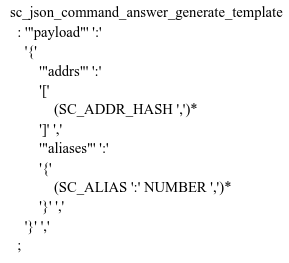
\includegraphics[scale=0.95]{images/generate_template_command_answer}}}
	\scnaddlevel{1}
		\scnsuperset{Язык описания грамматики языков ANTLR}
		\scnrelfromlist{интерпретация}{
			\scnfileitem{Сообщение \textit{ответа на команду создания sc-конструкции, изоморфной заданному sc-шаблону} состоит из списка найденных sc-конструкций и отображения псевдонимов sc-элементов на их позиции в тройках sc-шаблона. Ответ имеет статус 1, в случае успешной обработки команды.}
		}
	\scnaddlevel{-1}
	\scnrelfrom{изоморфизм}{ответ на команду создания sc-конструкции, изоморфной заданному sc-шаблону}
	\scnaddlevel{1}
		\scnidtf{search template command answer}
		\scnsuperset{ответ на команду на SC-JSON-коде}
		\scnsuperset{SC-JSON-код}
		\scnrelfrom{пример}{Пример ответа на команду создания sc-конструкции, изоморфной заданному sc-шаблону \\ \scneqfile{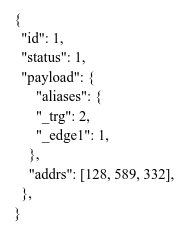
\includegraphics[scale=0.95]{images/generate_template_command_answer_example}}}
		\scnaddlevel{1}
			\scniselement{ответ на команду создания sc-конструкции, изоморфной заданному sc-шаблону}
			\scnrelfromlist{интерпретация}{
				\scnfileitem{Создана одна sc-конструкция, состоящая из одной тройки. Хеши sc-элементов в тройке: 128, 589, 332 соответственно их расположению в тройках. Команда выполнена успешно.}
			}
		\scnaddlevel{-1}
		\scnnote{Важно отметить, что sc-шаблон создания sc-конструкции не может быть пустым.}
	\scnaddlevel{-1}
\scnaddlevel{-1}

\scnhaselement{Правило написания сообщения \textit{команды поиска sc-конструкций, изоморфных заданному sc-шаблону,} и \textit{команды создания sc-конструкции, изоморфной заданному sc-шаблону}}
\scnaddlevel{1}
	\scnrelfrom{обобщённая структура}{\scnfileimage{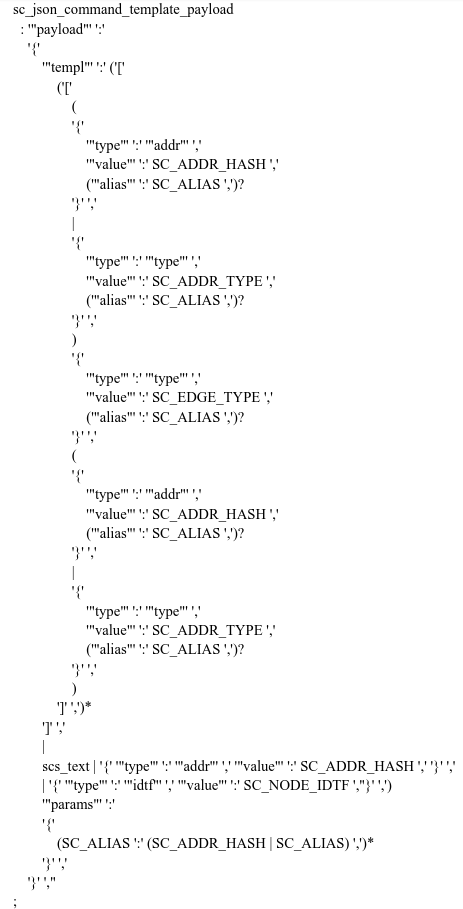
\includegraphics[scale=0.95]{images/template_message_command}}}
	\scnaddlevel{1}
		\scnsuperset{Язык описания грамматики языков ANTLR}
		\scnrelfromlist{интерпретация}{
			\scnfileitem{Сообщения \textit{команды поиска sc-конструкций, изоморфных заданному sc-шаблону,} и \textit{команды создания sc-конструкции, изоморфной заданному sc-шаблону} включают описание троек, необходимых для создания sc-шаблона поиска или генерации изоморфных sc-конструкций. Описание каждой тройки sc-шаблона включает описание sc-элементов этой тройки. Описания первого и третьего sc-элементов тройки должны всегда содержать хеш или тип в паре с ключевым словом "value". Если выбран тип, то в паре с ключевым словом "type"{} указывается "type"{}, если - хеш, то - "addr"{}. Вторым sc-элементом тройки должна быть дуга, для которой всегда указывается тип в паре с ключевым словом "value". Для каждого sc-элемента тройки может указываться псевдоним в паре с "alias". Псевдоним представляет собой строку и может быть использован для ассоциации с sc-элементами в других тройках sc-шаблона, либо ассоциации со значениями переменных sc-шаблона, которые указываются в списке под ключевым словом "params" и могут представлять собой либо хеш sc-элемента, либо его системный идентификатор. Таким образом, в некоторых случаях может отсутствовать необходимость указания хеша или типа sc-элемента. Также вместо списка описаний троек sc-шаблона, может указываться хеш или системный идентификатор sc-структуры, хранящейся в sc-памяти. Хеш и системный идентификатор указываются в паре с ключевым словом "value".}
		}
	\scnaddlevel{-1}
\scnaddlevel{-1}

\scnhaselement{Правило написания \textit{команды обработки sc-событий}}
\scnaddlevel{1}
	\scnrelfrom{обобщённая структура}{\scnfileimage{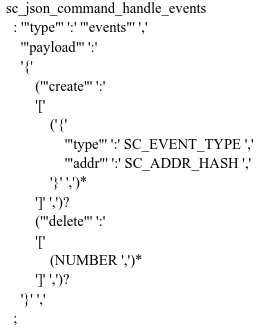
\includegraphics[scale=0.95]{images/handle_events_command}}}
	\scnaddlevel{1}
		\scnsuperset{Язык описания грамматики языков ANTLR}
		\scnrelfromlist{интерпретация}{
			\scnfileitem{Сообщение \textit{команды обработки sc-событий} может включать описание sc-элементов, по котором необходимо зарегистрировать или разрегистрировать sc-события. Идентификаторами подкоманд в описании команды могут быть "create"{} и "delete"{} соответственно, стоящие в паре с ключевым словом "command". Описание команды регистрации sс-cобытий "create"{} представляет собой список описаний типов sc-событий и sc-элементов, по которым необходимо зарегистрировать sc-события. Описания sc-элементов включают хеши этих sc-элементов в парах с ключевым словом "addr". Описание команды разрегистрации sc-событий представляет собой список позиций sc-событий в очереди sc-событий, которые необходимо удалить из этой очереди sc-событий.}
		}
	\scnaddlevel{-1}
	\scnsubset{Правило написания типов sc-событий}
	\scnaddlevel{1}
		\scnrelfrom{обобщённая структура}{\scnfileimage{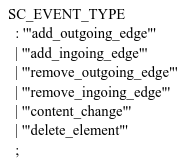
\includegraphics[scale=0.95]{images/sc_event_types}}}
		\scnaddlevel{1}
			\scnsuperset{Язык описания грамматики языков ANTLR}
			\scnrelfromlist{интерпретация}{
				\scnfileitem{Sc-событиями могут быть \textit{sc-события добавления выходящей дуги из sc-элемента (add\_outgoing\_edge)}, \textit{sc-события добавления входящей дуги в sc-элемент (add\_ingoing\_edge)}, \textit{sc-события удаления выходящей дуги из sc-элемента (remove\_outgoing\_edge)}, \textit{sc-события удаления входящей дуги в sc-элемент(remove\_ingoing\_edge)}, \textit{sc-события изменения содержимого sc-ссылки (content\_change)} и \textit{sc-события удаления sc-элемента (delete\_element)}.}
			}
		\scnaddlevel{-1}
	\scnaddlevel{-1}
	\scnrelfrom{изоморфизм}{команда обработки sc-событий}
	\scnaddlevel{1}
		\scnidtf{handle events command}
		\scnsuperset{команда на SC-JSON-коде}
		\scnsuperset{SC-JSON-код}
		\scnrelfrom{пример}{Пример команды обработки sc-событий \\ \scneqfile{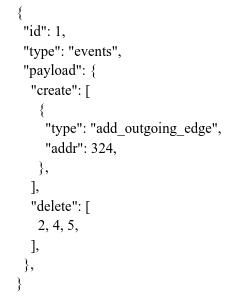
\includegraphics[scale=0.95]{images/handle_events_command_example}}}
		\scnaddlevel{1}
			\scniselement{команда обработки sc-событий}
			\scnrelfrom{ответ}{Пример ответа на команду обработки sc-событий}
			\scnrelfromlist{интерпретация}{
				\scnfileitem{(1) Зарегистрировать sc-событие типа "add\_outgoing\_edge"{} по sc-элементу с хешем 324; (2) Разрегистрировать sc-события с позициями sc-элементов 2, 4 и 5 соответственно.}
			}
		\scnaddlevel{-1}
		\scnrelfrom{ответная структура}{ответ на команду обработки sc-событий}
		\scnrelfrom{ответная структура}{ответ инициализации sc-события}
		\scnnote{\textit{Ответ инициализации sc-события} может производиться несколько раз за разные промежутки времени.}
	\scnaddlevel{-1}
\scnaddlevel{-1}

\scnhaselement{Правило написания \textit{ответа на команду обработки sc-событий}}
\scnaddlevel{1}
	\scnrelfrom{обобщённая структура}{\scnfileimage{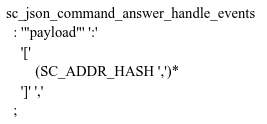
\includegraphics[scale=0.95]{images/handle_events_command_answer}}}
	\scnaddlevel{1}
		\scnsuperset{Язык описания грамматики языков ANTLR}
		\scnrelfromlist{интерпретация}{
		\scnfileitem{Сообщение \textit{ответа на команду обработки sc-событий} состоит из позиций зарегистрированных sc-событий в очереди. Успешным результатом \textit{команды обработки sc-событий} является статус 1.}
	}
	\scnaddlevel{-1}
	\scnrelfrom{изоморфизм}{ответ на команду обработки sc-событий}
	\scnaddlevel{1}
		\scnidtf{handle events command answer}
		\scnsuperset{ответ на команду на SC-JSON-коде}
		\scnsuperset{SC-JSON-код}
		\scnrelfrom{пример}{Пример ответа на команду обработки sc-событий \\ \scneqfile{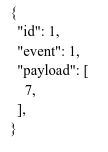
\includegraphics[scale=0.95]{images/handle_events_command_answer_example}}}
		\scnaddlevel{1}
			\scniselement{ответ на команду обработки sc-событий}
			\scnrelfromlist{интерпретация}{
				\scnfileitem{(1) Sc-событие типа "add\_outgoing\_edge"{} по sc-элементу с хешем 324 было зарегистрировано успешно на 7-ой позиции очереди sc-событий; (2) Sc-события под позициями 2, 4, 5 удалены успешно.}
			}
		\scnaddlevel{-1}
	\scnaddlevel{-1}
\scnaddlevel{-1}

\scnhaselement{Правило написания \textit{ответа инициализации sc-события}}
\scnaddlevel{1}
\scnrelfrom{обобщённая структура}{\scnfileimage{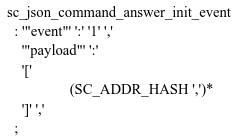
\includegraphics[scale=0.95]{images/init_event_command_answer}}}
\scnaddlevel{1}
\scnsuperset{Язык описания грамматики языков ANTLR}
\scnrelfromlist{интерпретация}{
	\scnfileitem{\textit{Ответ инициализации sc-события} возникает тогда и только тогда, когда в sc-памяти инициализируется соответствующее sc-событие. \textit{Ответ инициализации sc-события} всегда отсылается той клиентской системе, которая зарегистрировала это sc-событие. В сообщение \textit{ответа инициализации sc-события} включаются хеши тех sc-элементов, которые связаны с зарегистрированным sc-событием. Таким образом, если было зарегистрировано sc-событие выходящей sc-дуги, то в списке сообщения \textit{ответа инициализации sc-события} будут находится хеши трёх sc-элементов: хеш sc-элемента, который был подписан на sc-событие, хеш добавленной выходящей из него sc-дуги и хеш sc-элемента, являющегося концом этой sc-дуги.}
}
\scnaddlevel{-1}
\scnrelfrom{изоморфизм}{ответ инициализации sc-события}
\scnaddlevel{1}
\scnidtf{init event command answer}
\scnsuperset{ответ на команду на SC-JSON-коде}
\scnsuperset{SC-JSON-код}
\scnrelfrom{пример}{Пример ответа инициализации sc-события \\ \scneqfile{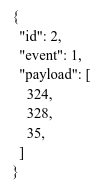
\includegraphics[scale=0.95]{images/init_event_command_answer_example}}}
\scnaddlevel{1}
\scniselement{ответ инициализации sc-события}
\scnrelfromlist{интерпретация}{
	\scnfileitem{Sc-событие было инициализировано успешно: добавлена выходящая sc-дуга с хешем 328 из зарегистрированного sc-элемента с хешем 324 в sc-элемент c хешем 35. Статус sc-события - 1.}
}
\scnaddlevel{-1}
\scnaddlevel{-1}
\scnaddlevel{-1}

\scnhaselement{Правило написания \textit{синтаксических типов sc-элементов}}
\scnaddlevel{1}
\scnrelfrom{обобщённая структура}{\scnfileimage{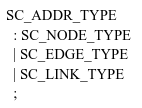
\includegraphics[scale=0.95]{images/sc_addr_types}}}
\scnaddlevel{1}
\scnsuperset{Язык описания грамматики языков ANTLR}
\scnrelfromlist{интерпретация}{
	\scnfileitem{\textit{Правило написания синтаксических типов sc-элементов} включает \textit{Правило написания синтаксических типов sc-узлов}, \textit{Правило написания синтаксических типов sc-дуг}, \textit{Правило написания синтаксических типов sc-ссылок}. Синтаксические типы sc-элементов представляются в виде целого числа и соответствуют программным синтаксическим типам, представляемым в sc-памяти.}
}
\scnaddlevel{-1}
\scnnote{На данный момент форма представления синтаксического типа sc-элемента зависит от того, как располагаются биты в маске sc-элемента. Следующим шагом в развитии \textit{SC-JSON-кода} и его грамматики могли быть стать устранение такой зависимости и переход к представлению синтаксических типов в виде строковых литералов, интерпретируемых \textit{Серверной системы на основе Websocket, обеспечивающей доступ к sc-памяти платформы интерпретации sc-моделей при помощи команд SC-JSON-кода}.}
\scnaddlevel{-1}

\scnhaselement{Правило написания \textit{синтаксических типов sc-узлов}}
\scnaddlevel{1}
\scnrelfrom{обобщённая структура}{\scnfileimage{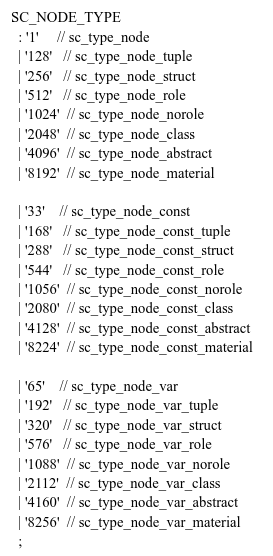
\includegraphics[scale=0.95]{images/sc_node_types}}}
\scnaddlevel{1}
\scnsuperset{Язык описания грамматики языков ANTLR}
\scnrelfromlist{интерпретация}{
	\scnfileitem{\textit{Правило написания синтаксических типов sc-узлов} описывает возможные синтаксические типы sc-узлов, интерпретируемые на стороне \textit{Серверной системы на основе Websocket, обеспечивающей доступ к sc-памяти платформы интерпретации sc-моделей при помощи команд SC-JSON-кода}.}
}
\scnaddlevel{-1}
\scnaddlevel{-1}

\scnhaselement{Правило написания \textit{синтаксических типов sc-дуг}}
\scnaddlevel{1}
\scnrelfrom{обобщённая структура}{\scnfileimage{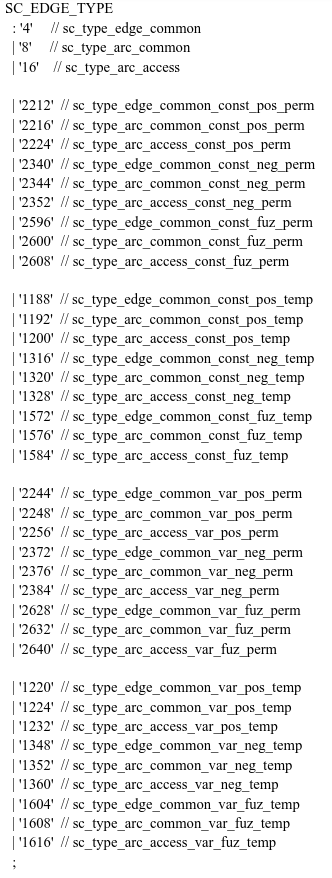
\includegraphics[scale=0.95]{images/sc_edge_types}}}
\scnaddlevel{1}
\scnsuperset{Язык описания грамматики языков ANTLR}
\scnrelfromlist{интерпретация}{
	\scnfileitem{\textit{Правило написания синтаксических типов sc-дуг} описывает возможные синтаксические типы sc-дуг, в том числе и sc-рёбер, интерпретируемые на стороне \textit{Серверной системы на основе Websocket, обеспечивающей доступ к sc-памяти платформы интерпретации sc-моделей при помощи команд SC-JSON-кода}.}
}
\scnaddlevel{-1}
\scnaddlevel{-1}

\scnhaselement{Правило написания \textit{синтаксических типов sc-ссылок}}
\scnaddlevel{1}
\scnrelfrom{обобщённая структура}{\scnfileimage{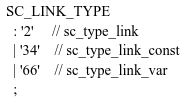
\includegraphics[scale=0.95]{images/sc_link_types}}}
\scnaddlevel{1}
\scnsuperset{Язык описания грамматики языков ANTLR}
\scnrelfromlist{интерпретация}{
	\scnfileitem{\textit{Правило написания синтаксических типов sc-ссылок} описывает возможные синтаксические типы sc-ссылок, интерпретируемые на стороне \textit{Серверной системы на основе Websocket, обеспечивающей доступ к sc-памяти платформы интерпретации sc-моделей при помощи команд SC-JSON-кода}.}
}
\scnaddlevel{-1}
\scnaddlevel{-1}

\scnendstruct \scninlinesourcecommentpar{Завершили представление \textit{Синтаксиса SC-JSON-кода}}

\scnheader{Серверная система на основе Websocket, обеспечивающая доступ к sc-памяти платформы интерпретации sc-моделей при помощи команд SC-JSON-кода}
\scnidtf{Система, работающая по принципам Websocket и предоставляющая параллельно-асинхронный многоклиентский доступ к sc-памяти платформы интерпретации sc-моделей при помощи SC-JSON-кода}
\scnidtf{SC-JSON-сервер}
\scntext{часто используемый неосновной внешний идентификатор sc-элемента}{SC-сервер}
\scnrelfromlist{используемый язык программирования}{C;C++}
\scnrelfromlist{используемый язык}{SC-JSON-код}
\scnexplanation{Стоит отметить, что текущая реализация \textit{Серверной системы на основе Websocket, обеспечивающая доступ к sc-памяти платформы интерпретации sc-моделей при помощи команд SC-JSON-кода} не является первой в своём роде и заменяет предыдущую её реализацию, написанную на языке Python. Причиной такой замены состоит в следующем:
	\begin{scnitemize}
		\item предыдущая реализация \textit{Серверной системы на основе Websocket, обеспечивающая доступ к sc-памяти платформы интерпретации sc-моделей при помощи команд SC-JSON-кода}, реализованная на языке программирования Python, зависит от библиотеки Boost Python, предоставляемой сообществом по развитию и коллаборации языков С++ и Python. Дело в том, что такое решение требует поддержки механизма интерпретации программного кода на языке Python на язык С++, что является избыточным и необоснованным, поскольку большая часть программного кода \textit{\textbf{Программного варианта реализации платформы интерпретации sc-моделей компьютерных систем}} реализована на языках С и С++. Новая реализация описываемой программной системы позволяет избавиться от использования ёмких и ресурсозатратных библиотек (например, boost-python-lib, llvm) и языка Python;
		\item при реализации распределённых подсистем важную роль играет скорость обработки знаний, то есть возможность быстро и срочно отвечать на запросы пользователя. Качество доступа к sc-памяти посредством реализованной \textit{Подсистемы взаимодействия с sc-памятью на основе языка JSON} должно быть соизмеримо с качеством доступа к sc-памяти при помощи специализированного программного интерфейса API, реализованного на том же языке программирования, что и сама система. Новая реализация позволяет повысить скорость обработки запросов \textit{Подсистемой взаимодействия с sc-памятью на основе языка JSON}, в том числе и обработка знаний, не менее чем в 1,5 раза по сравнению с предыдущим вариантом реализации этой подсистемы.
	\end{scnitemize}
}
\scnrelfrom{функциональная модель}{Модель \textit{Серверной системы на основе Websocket, обеспечивающая доступ к sc-памяти платформы интерпретации sc-моделей при помощи команд SC-JSON-кода}}
\scnaddlevel{1}
	\scnidtf{\large $elems^{elem\_types \;\; \times \;\; elem\_inc\_elems} \;\; \times \;\; elem\_types^{elems} \;\; \times \;\; \{\top, \bot\}^{elems} \;\; \times \;\; \\ keynodes^{elems} \;\; \times \;\; keynodes^{elem\_idtfs} \;\; \times \;\; \{\top, \bot\}^{keynodes} \;\; \times \;\; \\ link\_contents^{links} \;\; \times \;\; links^{link\_contents} \;\; \times \;\; \{\top, \bot\}^{links \;\; \times \;\; link\_contents} \;\; \times \;\; \\ elem\_structs^{elems\_types \;\; \times \;\; elems \;\; \times \;\; elem\_inc\_elems \;\; \times \;\; elem\_idtfs \;\; \times \;\; elem\_aliases} \;\; \times \;\; \\ \{\top, \bot\}^{elems\_structs} \;\; \times \;\; events^{elems \;\; \times \;\; event\_types} \;\; \times \;\; \{\top, \bot\}^{events}$}
	\scnexplanation{\textit{Модель Серверной системы на основе Websocket, обеспечивающая доступ к sc-памяти платформы интерпретации sc-моделей при помощи команд SC-JSON-кода} описывает необходимы и достаточный программный интерфейс для взаимодействия c sc-памятью. В общем случае описывает функциональные возможности не только \textit{Серверной системы на основе Websocket, обеспечивающая доступ к sc-памяти платформы интерпретации sc-моделей при помощи команд SC-JSON-кода}, но клиентских систем взаимодействующих с ней, поскольку зачастую эти клиентские системы включают специализированный программный интерфейс, схожий с интерфейсом серверной системы, но на другом языке программирования.}
	\scneqtoset{
		функция создания sc-элементов по их описаниям: типам и инцидентным sc-элементам*\\
		\scnaddlevel{1}
			\scnidtf{\large $elems^{elem\_types \times elem\_inc\_elems}$}
			\scnnote{Каждый sc-элемент из множества elems имеет соответствующий синтаксический тип из множества elem\_types и возможно связан с sc-элементами из множества elem\_inc\_elems.}
		\scnaddlevel{-1};
		функция получения соответствующих синтаксических типов sc-элементов*\\
		\scnaddlevel{1}
			\scnidtf{\large $elem\_types^{elems}$}
			\scnnote{У каждого sc-элемента из множества elems можно получить соответствующий синтаксический тип из множества elem\_types.}
		\scnaddlevel{-1};
		функция проверки существования sc-элементов в sc-памяти*\\
		\scnaddlevel{1}
			\scnidtf{\large $\{\top, \bot\}^{elems}$}
			\scnnote{Каждый sc-элемент из множества elems должен находиться в sc-памяти.}
		\scnaddlevel{-1};
		функция получения ключевого sc-элемента по системному идентификатору*\\
		\scnaddlevel{1}
			\scnidtf{\large$(keynodes^{elems} \;\; \cup \;\; keynodes^{elem\_idtfs}) \;\; / \;\;$ \normalsize \textit{функция разрешения ключевого sc-элемента по системному идентификатору*}}
			\scnnote{Каждый ключевой sc-элемент из множества keynodes является sc-элементом множества elems и имеет, по крайней мере, системный идентификатор из множества elem\_idtfs.}
		\scnaddlevel{-1};
		функция разрешения ключевого sc-элемента по системному идентификатору*\\
		\scnaddlevel{1}
			\scnidtf{\large $(keynodes^{elems} \;\; \cup \;\; keynodes^{elem\_idtfs}) \;\; / \;\;$ \normalsize \textit{функция получения ключевого sc-элемента по системному идентификатору*}}
			\scnnote{Из каждого sc-элемента множества elems можно получить ключевой sc-элемент множества keynodes, зная, по крайней мере, его системный идентификатор из множества elem\_idtfs.}
		\scnaddlevel{-1};
		функция установки содержимого в sc-cсылки*\\
		\scnaddlevel{1}
			\scnidtf{\large $\{\top, \bot\}^{links \;\; \times \;\; link\_contents}$}
			\scnnote{В каждый sc-элемент из множества sc-ccылок links может быть установлено содержимое из множества link\_contents.}
		\scnaddlevel{-1};
		функция получения содержимого из sc-ссылок*\\
		\scnaddlevel{1}
			\scnidtf{$link\_contents^{links}$}
			\scnnote{Из каждый sc-элемент из множества sc-ccылок links можно получить содержимое, принадлежащее множеству link\_contents.}
		\scnaddlevel{-1};
		функция получения sc-ccылок по содержимому*\\
		\scnaddlevel{1}
			\scnidtf{\large $links^{link\_contents}$}
			\scnnote{По содержимому из множества link\_contents можно получить подмножество sc-ссылок из множества links, в которые установлено это содержимое.}
		\scnaddlevel{-1};
		функция поиска sc-конструкций, изоморфных заданному sc-шаблону, состоящего из троек, специфицированных инцидентными sc-элементами и/или синтаксическими типами и/или идентификаторами и/или псевдонимами их sc-элементов*\\
		\scnaddlevel{1}
			\scnidtf{$elem\_structs^{elems\_types \;\; \times \;\; elems \;\; \times \;\; elem\_inc\_elems \;\; \times \;\; elem\_idtfs \;\; \times \;\; elem\_aliases} \;\; \times \;\; \\ \{\top, \bot\}^{elems\_structs} \;\; / \;\;$ \normalsize \textit{функция создания sc-конструкции, изоморфной заданному sc-шаблону, состоящего из троек, специфицированных инцидентными sc-элементами и/или синтаксическими типами и/или идентификаторами и/или псевдонимами их sc-элементов*}}
			\scnnote{По синтаксическим типам sc-элементов из множества elems\_types и/или sc-элементам из множества elems, связанными с sc-элементами, у которых известны синтаксические типы из множества elems\_types, в том числе инцидентным из множества elem\_inc\_elems, и/или системный идентификаторам sc-элементов множества elem\_idtfs и/или псевдонимам этих sc-элементов множества  elem\_aliases могут быть получены соответствующие фрагменты базы знаний множества elem\_structs, состояющие из всех этих sc-элементов.}
		\scnaddlevel{-1};
		функция создания sc-конструкции, изоморфной заданному sc-шаблону, состоящего из троек, специфицированных инцидентными sc-элементами и/или синтаксическими типами и/или идентификаторами и/или псевдонимами их sc-элементов*\\
		\scnaddlevel{1}
			\scnidtf{$elem\_structs^{elems\_types \;\; \times \;\; elems \;\; \times \;\; elem\_inc\_elems \;\; \times \;\; elem\_idtfs \;\; \times \;\; elem\_aliases} \;\; / \;\;$ \normalsize \textit{функция поиска sc-конструкций, изоморфных заданному sc-шаблону, состоящего из троек, специфицированных инцидентными sc-элементами и/или синтаксическими типами и/или идентификаторами и/или псевдонимами их sc-элементов*}}
			\scnnote{По синтаксическим типам sc-элементов из множества elems\_types и/или sc-элементам из множества elems, связанными с sc-элементами, у которых известны синтаксические типы из множества elems\_types, в том числе инцидентным из множества elem\_inc\_elems, и/или системный идентификаторам sc-элементов множества elem\_idtfs и/или псевдонимам этих sc-элементов множества  elem\_aliases всегда можно создать фрагмент базы знаний множества elem\_structs, состояющий из всех этих sc-элементов.}
		\scnaddlevel{-1};
		функция регистрации sc-события в виде sc-элемента\\
		\scnaddlevel{1}
			\scnidtf{$events^{elems \;\; \times \;\; event\_types}$}
			\scnnote{На каждый sc-элемент множества elems можно подписать sc-cобытие из множества events типа из множества event\_types.}
		\scnaddlevel{-1};
		функция разрегистрации sc-события в виде sc-элемента\\
		\scnaddlevel{1}
			\scnidtf{$\{\top, \bot\}^{events}$}
			\scnnote{На каждый sc-элемент множества elems можно отписать от sc-cобытия из множества events.}
		\scnaddlevel{-1}
	}
\scnaddlevel{-1}
\scnrelfromlist{характеристика}{
	\scnfileitem{\textit{Серверная система на основе Websocket, обеспечивающая доступ к sc-памяти платформы интерпретации sc-моделей при помощи команд SC-JSON-кода}}
}

\bigskip
\scnendstruct \scninlinesourcecommentpar{Завершили описание \textit{Подсистемы взаимодействия c sc-памятью на основе языка JSON}}

\bigskip
\end{scnsubstruct} \scnendsegmentcomment{\textit{Описание реализации подсистемы взаимодействия с внешней средой с использованием сетевых языков}}
